\documentclass[10pt]{beamer}
\usetheme[
%%% options passed to the outer theme
%    hidetitle,           % hide the (short) title in the sidebar
     hideauthor,          % hide the (short) author in the sidebar
%    hideinstitute,       % hide the (short) institute in the bottom of the sidebar
%    shownavsym,          % show the navigation symbols
%    width=2cm,           % width of the sidebar (default is 2 cm)
%    hideothersubsections,% hide all subsections but the subsections in the current section
%    hideallsubsections,  % hide all subsections
    left               % right of left position of sidebar (default is right)
%%% options passed to the color theme
%    lightheaderbg,       % use a light header background
]{AAUsidebar}

% If you want to change the colors of the various elements in the theme, edit and uncomment the following lines
% Change the bar and sidebar colors:
\definecolor{spartanBlue}{RGB}{0,85,162}
\definecolor{spartanYellow}{RGB}{229,168,35}
\definecolor{spartanGray}{RGB}{147,149,151}
\definecolor{darkGreen}{RGB}{34, 139, 34}

\setbeamercolor{frametitle}{use=structure,fg=white,bg=spartanBlue}
\setbeamercolor{title}{fg=frametitle.bg}

\setbeamercolor{header}{bg=spartanBlue}

\setbeamercolor{title in sidebar}{fg=frametitle.bg} % Headings on the side bar
\setbeamercolor{palette sidebar secondary}{fg=frametitle.bg} % Headings on the side bar
%\setbeamercolor{palette sidebar primary}{fg=frametitle.bg} % Slide titles (i.e., not slide sections)

\setbeamercolor{section in toc}{use=palette sidebar secondary,fg=palette sidebar secondary.fg} 
\setbeamercolor{subsection in toc}{use=normal text,fg=palette normal text.fg} 
\setbeamercolor{block title}{fg=spartanBlue} % Color of headings
\setbeamercolor{local structure}{fg=spartanBlue} % Color of enumerated items (e.g. lists, bullets, etc.)
\setbeamercolor{bibliography item}{use=local structure,fg=local structure.fg} % Color number of bibliography items
\setbeamercolor{bibliography entry author}{use=normal text,fg=normal text.fg} % Color bibliography entry.  Includes not just author but all fields


\usepackage{environ}
\usepackage{tikz}
\usepackage{algorithm}
\usepackage[noend]{algpseudocode}
\usepackage{listings} % Used for printing source code in papers
\usepackage{pgfplots} % Used to create graphs
\usepackage{makecell} % Used to create thick links in tables
\usepackage{algorithm} % Used for writing algorithms in a paper
\usepackage[noend]{algpseudocode} % Allows psuedocode keywords (e.g., "if", "while", "for", etc.) in algorithms.
\usepackage{xcolor, colortbl} % Used for coloring the cells of tables
\usepackage[utf8]{inputenc}
\usepackage[english]{babel}
\usepackage[T1]{fontenc}
% Or whatever. Note that the encoding and the font should match. If T1
% does not look nice, try deleting the line with the fontenc.
\usepackage{helvet}

% colored hyperlinks
\newcommand{\chref}[2]{%
  \href{#1}{{\usebeamercolor[bg]{AAUsidebar}#2}}%
}

\title[A Fully-Automated Solver for Multiple Square Jigsaw Puzzles Using Hierarchical Clustering]% optional, use only with long paper titles
{\textbf{A Fully-Automated Solver for Multiple Square Jigsaw Puzzles Using Hierarchical Clustering}}

\subtitle{}  % could also be a conference name

\date{October 27, 2016}

\author[Zayd Hammoudeh] % optional, use only with lots of authors
{
    Zayd Hammoudeh\\
    \href{mailto:hammoudeh@gmail.com}{{\tt hammoudeh@gmail.com}}
}
% - Give the names in the same order as they appear in the paper.
% - Use the \inst{?} command only if the authors have different
%   affiliation. See the beamer manual for an example

\institute[
%  {\includegraphics[scale=0.2]{aau_segl}}\\ %insert a company, department or university logo
    Dept.\ of Computer Science\\
    San Jose State University\\
] % optional - is placed in the bottom of the sidebar on every slide
{% is placed on the title page
    Department of Computer Science\\
    San Jose State University\\
  
  %there must be an empty line above this line - otherwise some unwanted space is added between the university and the country (I do not know why;( )
}


% specify a logo on the titlepage (you can specify additional logos an include them in 
% institute command below
\pgfdeclareimage[height=1.5cm]{titlepagelogo}{images/SJSU_Seal_Blue} % placed on the title page
\titlegraphic{% is placed on the bottom of the title page
  \pgfuseimage{titlepagelogo}
%  \hspace{1cm}\pgfuseimage{titlepagelogo2}
}


%%%%%%%%%%%%%%%%%%%%%%%%%%%%%%%%%%%%%%%%%%
%% Handles Slide Numbering For Appendix %%
%%%%%%%%%%%%%%%%%%%%%%%%%%%%%%%%%%%%%%%%%%
\newcommand{\backupbegin}{
   \newcounter{finalframe}
   \setcounter{finalframe}{\value{framenumber}}
}
\newcommand{\backupend}{
   \setcounter{framenumber}{\value{finalframe}}
}
%%%%%%%%%%%%%%%%%%%%%%%%%%%%%%%%%%%%%%%%%%


%%%%%%%%%%%%%%%%%%%%%%%%%%%%%%%%%%%%%%%%%%
%%   Scales tikz images to side size    %%
%%%%%%%%%%%%%%%%%%%%%%%%%%%%%%%%%%%%%%%%%%
\makeatletter
\newsavebox{\measure@tikzpicture}
\NewEnviron{scaletikzpicturetowidth}[1]{%
  \def\tikz@width{#1}%
  \def\tikzscale{1}\begin{lrbox}{\measure@tikzpicture}%
  \BODY
  \end{lrbox}%
  \pgfmathparse{#1/\wd\measure@tikzpicture}%
  \edef\tikzscale{\pgfmathresult}%
  \BODY
}
\makeatother
%%%%%%%%%%%%%%%%%%%%%%%%%%%%%%%%%%%%%%%%%%



\begin{document}
% the titlepage
{
\begin{frame}[plain,noframenumbering]{}{} % the plain option removes the sidebar and header from the title page
	\titlepage
\end{frame}}
%%%%%%%%%%%%%%%%



%% TOC
%\begin{frame}{Agenda}{}
%	\tableofcontents
%\end{frame}
%%%%%%%%%%%%%%%%%



\section{Introduction}
\begin{frame}{Introduction}{Jigsaw Puzzles}
  \begin{itemize}
    \item First jigsaw puzzle introduced in the 1760s.  Modern jigsaw puzzles were introduced in the 1930s.
    \vfill
    \item First computation jigsaw puzzle solver introduced in 1964.
    \vfill
    \item Solving a jigsaw puzzle is NP Complete \cite{altman1990, demaine2007}
    \vfill
    \item<2-> \textbf{Example Applications:} DNA fragment reassembly, shredded document reconstruction, speech descrambling, and image editing.
    \begin{itemize}
        \item<3-> In most cases, the original, ``ground-truth'' image is unknown.
    \end{itemize}
  \end{itemize}
\end{frame}
%%%%%%%%%%%%%%%%


\begin{frame}{Introduction}{Jig Swap Puzzles}
    \textbf{Jigswap Puzzles} -- Variant of the traditional jig saw puzzle
    \begin{itemize}
        \item All pieces are equal-sized squares
        \item Substantially more difficult
    \end{itemize}
    \vfill
    % Delay the table on the slide
    \begin{tabular}{ >{\centering\arraybackslash}m{0.45\textwidth} >{\centering\arraybackslash}m{0.45\textwidth} }
	\onslide<2->{\fbox{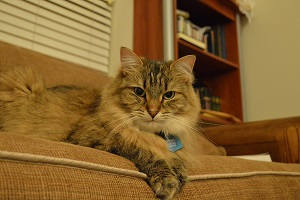
\includegraphics[width=0.365\textwidth]{./images/muffins_300x200.jpg}}} & \onslide<3->{\fbox{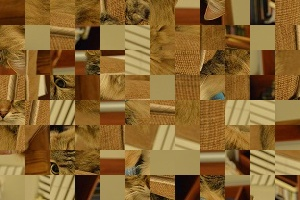
\includegraphics[width=0.365\textwidth]{./images/muffins_scrambled.jpg}}}
	\\ ~\\
	\onslide<2->{Ground-Truth Image} & \onslide<3->{Randomized Jig Swap Puzzle}
	\\ ~\\
  \end{tabular}
\end{frame}
%%%%%%%%%%%%%%%%



\begin{frame}{Introduction}{Jig Swap Puzzle Types}
\onslide<2->{There are four primary jig swap puzzle types as formalized by~\cite{gallagher2012}. In all cases, the ``ground-truth'' input(s) is unknown.} 
    \vfill
    \begin{itemize}
        \item<2-> \textbf{Type~1}: Puzzle dimension and piece rotation are known.  One or more ``anchor'' pieces are fixed in their correct location.
        \vfill
        \item<3-> \textbf{Type~2}: All piece locations and rotations unknown.  Puzzle dimensions may be known.
        \vfill
        \item<4-> \textbf{Type~3}: All piece locations are known.  Only rotation is unknown.
        \vfill
        \item<5-> \textbf{Mixed-Bag}: Pieces come from multiple puzzles.
    \end{itemize}
    \vfill
    \onslide<6->{Mixed-Bag Puzzles are the focus of this thesis.}
\end{frame}
%%%%%%%%%%%%%%%%



\begin{frame}{Introduction}{Best Buddies}\label{frame:bestBuddies}
    \begin{itemize}
        \item \textbf{Basis of all Modern Jig Swap Solvers}: The more compatible two pieces are on their respective sides, the more likely they are to be adjacent.
        \vfill
        \item \textbf{Best Buddies}: Any pair of puzzles pieces that are more compatible with each other on their respective sides than they are to any other piece~\cite{pomeranz2011}
        \vfill
\begin{equation} \label{eq:pomeranzBestBuddyDefinition}
\centering
\begin{split}
	\begin{matrix}
		\forall{p_{k}}\forall{s_z},C(p_i, s_x, p_j, s_y) \geq C(p_i, s_x, p_k, s_z)
		\\
		\\
		\textnormal{and}
		\\
		\\
		\forall{p_{k}}\forall{s_z},C(p_j, s_y, p_i, s_x) \geq C(p_j, s_y, p_k, s_z)
	\end{matrix}
\end{split}
\end{equation} 
        \vfill
        \item \textbf{Importance of Best Buddies}: Strong indicator of piece adjacency
    \end{itemize}
\end{frame}
%%%%%%%%%%%%%%%%



\subsection{Previous Work}
\begin{frame}{Previous Work}{}
    \begin{itemize}
        \onslide<1->{\item \textbf{Cho \textit{et al.}}~\cite{cho2010} -- Introduced the first Modern Jig Swap Puzzle Solver Introduced
        \begin{itemize}
            \setlength\itemsep{.8em}
            \item Graphical model-based Type~1 solver
            \item Puzzle dimensions are known
            \item Used one or more anchor pieces
            \item Established the standard test conditions including puzzle piece size and image encoding using the LAB~colorspace
        \end{itemize}}
        \vfill
        \onslide<2->{\item \textbf{Pomeranz \textit{et al.}}~\cite{pomeranz2011} -- Iterative, greedy jigsaw Type~1 puzzle solver
        \begin{itemize}
            \setlength\itemsep{.8em}
            \item Eliminated the use of anchor pieces 
            \item Created multiple solver benchmarks of various sizes
            \item Introduced the concept of ``best buddies''
        \end{itemize}}
    \end{itemize}
\end{frame}
%%%%%%%%%%%%%%%%



\section{Mixed-Bag Solver}
\begin{frame}{Mixed-Bag Solver}{Solving a Jigsaw Puzzle}
	\onslide<1->{\begin{block}{\textbf{Paikin~\& Tal's Algorithm}} 
	    \begin{itemize}
        \setlength\itemsep{.8em}
		    \item Begin each puzzle with a single distinct piece
		    \item Place all pieces around the expanding core
	    \end{itemize}
	\end{block}}
	\vfill
	\onslide<2->{\begin{block}{\textbf{Alternate Jigsaw Puzzle Solving Strategy}}
    \begin{itemize}
      \setlength\itemsep{.8em}
			\item Correctly assemble small puzzle regions (i.e., segments)
			\item Iteratively merge smaller regions to form large ones	
			\onslide<3->{\item \textbf{Advantage of this Approach}: 
			\begin{itemize}
			    \setlength\itemsep{.8em}
			    \item Reduces the size of the problem
			    \item Provides structure to the unordered set of puzzle pieces.
			\end{itemize}}
    \end{itemize}
	\end{block}}
	\vfill
  \onslide<4->{This alternate strategy is the basis of the \textbf{Mixed-Bag Solver}.}
\end{frame}

\subsection{Assembler}
\subsection{Segmentation}
\subsection{Stitching}
\subsection{Hierarchical Clustering}
\subsection{Final Seed Piece Selection}
\subsection{Final Assembly}

\section{Quantifying Quality}
\subsection{Direct Accuracy}
\subsection{Neighbor Accuracy}



\subsection{Best Buddy Density}
\begin{frame}{Quantifying Solver Quality}{Best Buddy Density}
  \begin{itemize}
    \setlength\itemsep{1em}
    \item \textbf{Best Buddies Review}: Any pair of puzzles pieces that are more compatible with each other on their respective sides than they are to any other piece
    \begin{itemize}
      \item \textbf{Note}: Not all puzzle pieces will have a best buddy.
    \end{itemize}
    \vfill
    \item \textbf{Best Buddy Density} (BBD): A metric for quantifying the best buddy profile of an image that is independent of image size.
    \vfill
    \begin{equation} \label{eq:bestBuddyDensity}
      BBD = \frac{b}{n \cdot q}
    \end{equation}
    \vfill
    \item A greater BBD means the pieces are more differentiated making the puzzle easier to solve.
  \end{itemize}
\end{frame}
%%%%%%%%%%%%%%%%



\begin{frame}{Quantifying Solver Quality}{Best Buddy Density}  
  \begin{block}{\textbf{Visualizing Best Buddy Density}}
    \begin{itemize}
      \setlength\itemsep{1em}
      \item Transform each puzzle piece into a square consisting of four isosceles triangles.
      \item Color each triangle according to whether the adjacent piece is a best buddy.  The scheme used in this thesis:
    \end{itemize}
    \begin{table}
      \begin{center}
        \begin{tabular}{ | >{\centering\arraybackslash}m{0.62in} | >{\centering\arraybackslash}m{0.78in} | >{\centering\arraybackslash}m{0.7in} | >{\centering\arraybackslash}m{0.62in} | }
              
          \hline
          {\small No Best Buddy} & {\small Non-Adjacent Best Buddy} & {\small Adjacent Best Buddy} & {\small No Piece Present}  \\ \hline
          {\cellcolor{white}~} & {\cellcolor{red}~} & {\cellcolor{green}~} & {\cellcolor{black}~}  \\
          {\cellcolor{white}~} & {\cellcolor{red}~} & {\cellcolor{green}~} & {\cellcolor{black}~}  \\
          \hline
        \end{tabular}
      \end{center}
    \end{table}
    \begin{itemize}
      \setlength\itemsep{1em}
      \item Areas with higher best buddy density will have more green triangles.
    \end{itemize}
  \end{block}
\end{frame}
%%%%%%%%%%%%%%%%



\begin{frame}{Quantifying Solver Quality}{Example Visualizing Best Buddy Density}  

\begin{figure}[t]
  \centering
  \begin{tabular}{ >{\centering\arraybackslash}m{0.40\textwidth} >{\centering\arraybackslash}m{0.40\textwidth} }
     \onslide<1->{\fbox{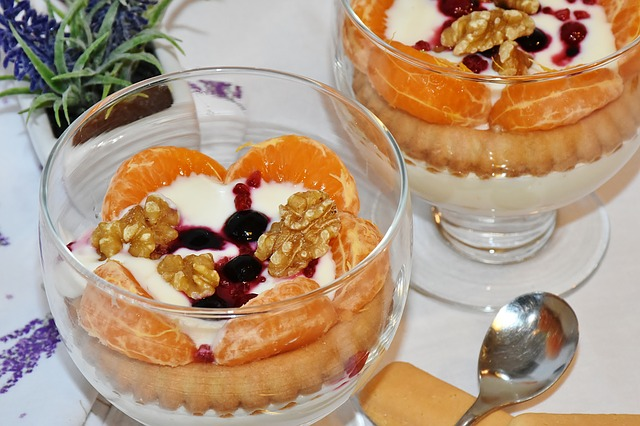
\includegraphics[width=0.37\textwidth]{./images/dessert_pixabay.jpg}}}  & \onslide<2->{\fbox{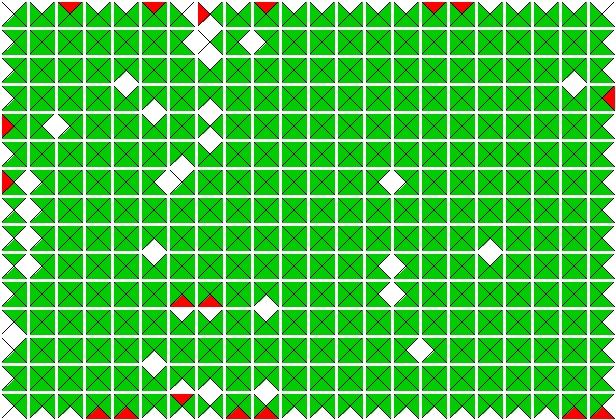
\includegraphics[width=0.37\textwidth]{./images/dessert_best_buddy_visualization.jpg}}}
     \\~\\
     \onslide<1->{(a) Original Image~\cite{pixabay}} & \onslide<2->{(b) Best Buddy Visualization}
  \end{tabular}
\onslide<1->{\caption{Visualization of Best Buddy Density}}
\label{fig:bestBuddyVisualization}
\end{figure}

\end{frame}
%%%%%%%%%%%%%%%%




\section{Experimental Results}
\begin{frame}{Experimental Results}{Determining Input Puzzle Count}
  \begin{itemize}
    \onslide<1->{\item \textbf{Goal}: Measure the Mixed-Bag Solver's accuracy determining the number of input puzzles}
      \vspace{0.4em}
      \begin{itemize}
        \item \textbf{Importance} -- The Mixed-Bag Solver must estimate this accurately to provide meaningful outputs.
      \end{itemize}
    \vfill
    \onslide<2->{\textbf{Two Subexperiments}:
      \vspace{0.4em}
      \begin{itemize}
        \item \textbf{Single Puzzle Accuracy} -- This represents the solver's performance ceiling
        \item \textbf{Multiple Puzzle Accuracy} -- A more general estimate of the solver's performance
      \end{itemize}
    }
  \end{itemize}
\end{frame}
%%%%%%%%%%%%%%%%



\subsection{Input Puzzle Count}
\begin{frame}{Experimental Results}{Determining Input Puzzle Count}

\end{frame}
%%%%%%%%%%%%%%%%



\begin{frame}{Determining Input Puzzle Count}{Comparison of Best Buddy Density for Misclassified Images}
  \begin{tabular}{ >{\centering\arraybackslash}m{0.45\textwidth} >{\centering\arraybackslash}m{0.45\textwidth} }

	\onslide<1->{\fbox{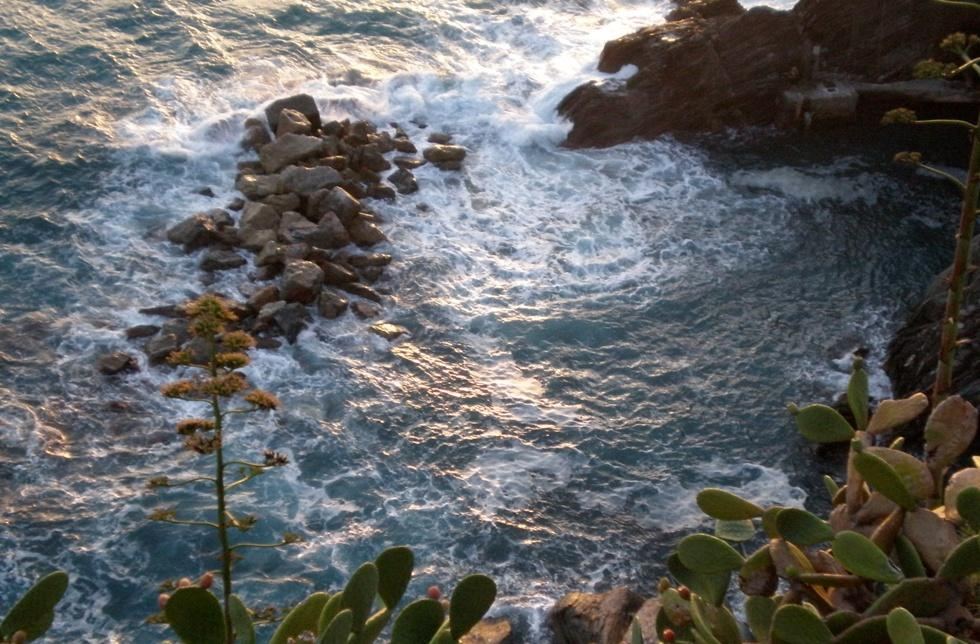
\includegraphics[width=0.35\textwidth]{./images/single_puzzle/pomeranz_805_14.jpg}}} & \onslide<2->{\fbox{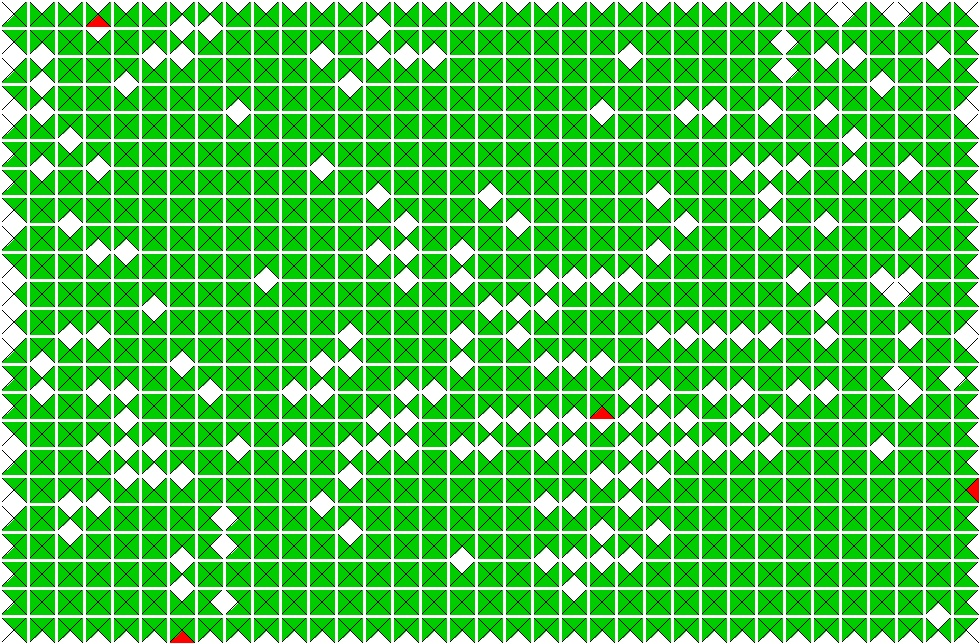
\includegraphics[width=0.35\textwidth]{./images/single_puzzle/best_buddies_pomeranz_805_14.jpg}}} \\~\\
	\onslide<1->{\small Perfectly Reconstructed Image~(a)} & \onslide<2->{\small Best Buddy Visualization~(a) }
\\~\\
	\onslide<1->{\fbox{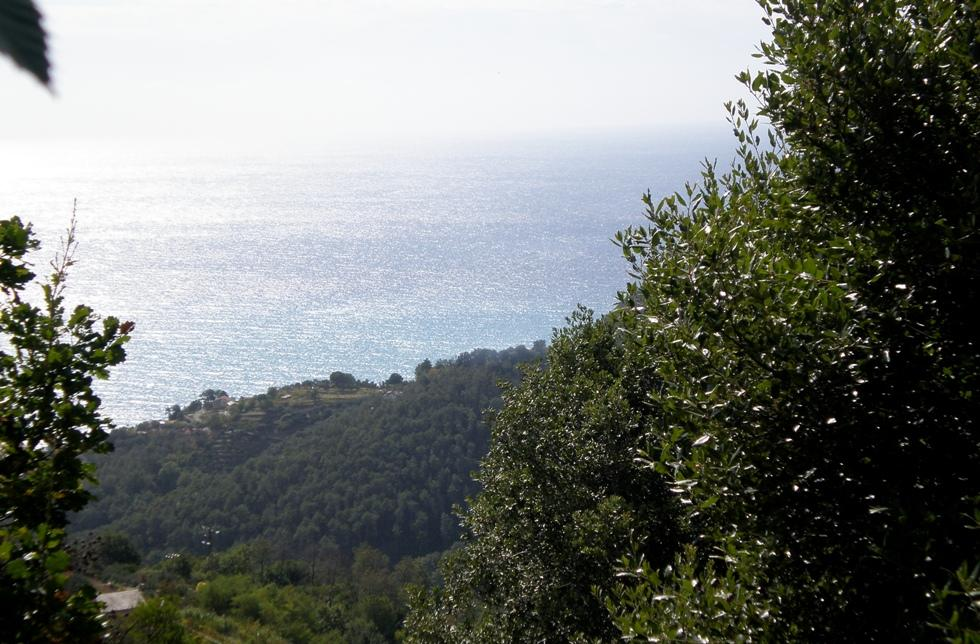
\includegraphics[width=0.35\textwidth]{./images/single_puzzle/pomeranz_805_12.jpg}}} & \onslide<2->{\fbox{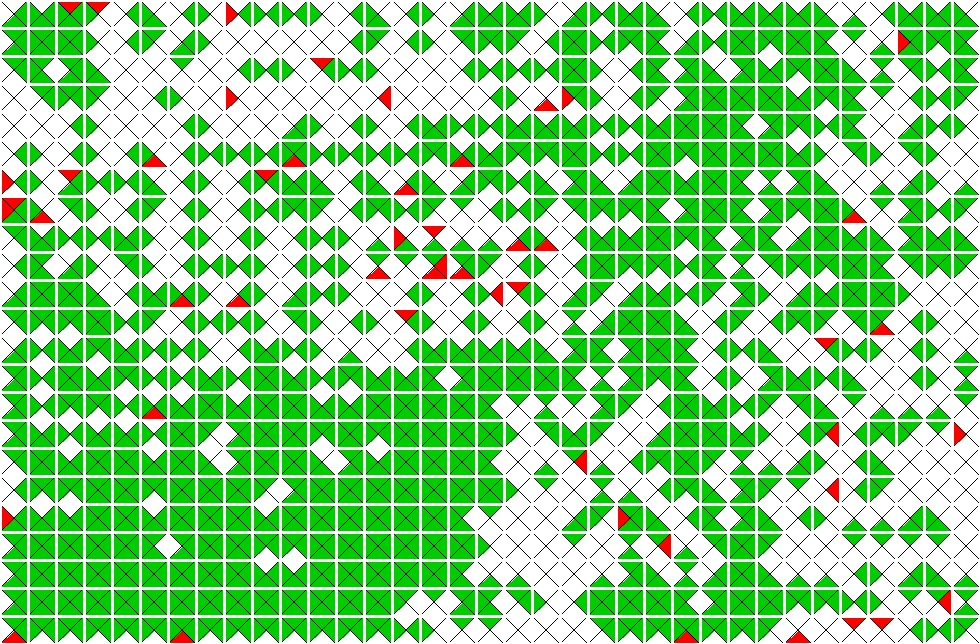
\includegraphics[width=0.35\textwidth]{./images/single_puzzle/best_buddies_pomeranz_805_12.jpg}}} \\~\\
	\onslide<1->{\small Misclassified Image~(b)} & \onslide<2->{\small Best Buddy Visualization~(b)}
  \end{tabular}
\end{frame}
%%%%%%%%%%%%%%%%



\begin{frame}{Determining Input Puzzle Count}{Multiple Input Puzzles}
     \begin{center}
       \begin{scaletikzpicturetowidth}{0.9\textwidth}
        \begin{tikzpicture}[scale=\tikzscale]
          \begin{axis}[
                ybar, axis on top,
                height=8cm, width=12cm,
            	axis background/.style={fill=gray!10},
                bar width=0.4cm,
                ymajorgrids, tick align=inside,
                major grid style={draw=white},
                enlarge y limits={value=.1,upper},
                ymin=0, ymax=100,
                axis x line*=bottom,
                axis y line*=left,
                y axis line style={opacity=1},
                tickwidth=0pt,
                title=\textbf{Mixed-Bag Solver's Input Puzzle Count Error Frequency},
                enlarge x limits=0.2,
                legend style={
                    at={(0.5,-0.2)},
                    anchor=north,
                    legend columns=-1,
                    /tikz/every even column/.append style={column sep=0.5cm}
                },
                xlabel={Size of Input Puzzle Count Error},
                ylabel={Frequency (\%)},
                symbolic x coords={
                   0, 1, 2, 3},
               xtick=data,
               nodes near coords={
                \pgfmathprintnumber[precision=0]{\pgfplotspointmeta}
               }
            ]
        \addplot [fill=blue!30]
            coordinates {(0,74.5) (1,16.4) (2,7.3) (3,1.8)};
        \addplot [fill=red!30]
            coordinates {(0,44) (1,48) (2,4) (3,4)};
        \addplot [fill=green!30]
            coordinates {(0,50) (1,50) (2,0) (3,0)};
        \addplot [fill=gray]
            coordinates {(0,60) (1,20) (2,20) (3,0)};
        \legend{2 Puzzles, 3 Puzzles, 4 Puzzles, 5 Puzzles}
        \end{axis}
        \end{tikzpicture}
      \end{scaletikzpicturetowidth}  
    \end{center}
\end{frame}
%%%%%%%%%%%%%%%%



\subsection{Solver Comparison}
\begin{frame}{Experimental Results}{Performance Comparison on Multiple Input Puzzles}

  \begin{itemize}
    \onslide<1->{\item \textbf{Goal}: Compare the performance of the Mixed-Bag Solver and Paikin~\& Tal's algorithm 
    \vfill
    \item \textbf{Procedure:} Randomly select, without replacement, a specified number of images and input them into both solvers.
    \vfill
    \item \textbf{Metrics Used}:
    \begin{itemize}
      \item Shiftable Enhanced Direct Accuracy Score (SEDAS)
      \item Enhanced Neighbor Accuracy Score (ENAS)
      \item Perfect Reconstruction Percentage
    \end{itemize}}
    \vfill
    \onslide<2->{\item \textbf{Note}: The Mixed-Bag Solver's results are subdivided according to whether the number of input puzzles was estimated correctly.
    \begin{itemize}
      \item This estimates the performance ceiling if hierarchical clustering performs optimally.}
    \end{itemize}
  \end{itemize}

\end{frame}
%%%%%%%%%%%%%%%%



\begin{frame}{Comparison of Solver Performance}{Shiftable Enhanced Direct Accuracy Score (SEDAS)}
     \begin{center}
       \begin{scaletikzpicturetowidth}{0.9\textwidth}
        \begin{tikzpicture}[scale=\tikzscale]
          \begin{axis}[
            height=8cm, width=12cm,
            axis background/.style={fill=gray!10},
            title=\textbf{Effect of the Number of Input Puzzles on SEDAS},
            xlabel={\textbf{Number of Input Puzzles}},
            ylabel={\textbf{SEDAS}},
            xmin=1.5, xmax=5.5,
            ymin=0, ymax=1,
            xtick={2, 3, 4, 5},
            ytick={0,0.2,0.4,0.6,0.8,1.0},
            ymajorgrids=true,
            grid style=dashed,
            legend style={ at={(0.5,-0.25)}, anchor=north, legend columns=-1, /tikz/every even column/.append style={column sep=0.5cm}}
            ]
        \addplot [color=blue,mark=*,mark options={fill=blue},ultra thick]
            coordinates {(2,0.849835) (3,0.953583)
                 (4,0.88068) (5,0.792796)};
        \addplot [color=red,mark=square*,mark options={fill=red},ultra thick]
            coordinates {(2,0.757159) (3,0.799822)
                 (4,0.777987) (5,0.782815)};
        \addplot [color=darkGreen,mark=triangle*,mark options={fill=darkGreen},ultra thick]
            coordinates {(2,0.321232) (3,0.202879)
                 (4,0.108857) (5,0.09866)};
        \legend{MBS Correct Puzzle Count, MBS All, Paikin \& Tal}
        \end{axis}
        \end{tikzpicture}
      \end{scaletikzpicturetowidth}  
    \end{center}
\end{frame}
%%%%%%%%%%%%%%%%



\begin{frame}{Comparison of Solver Performance}{Enhanced Neighbor Accuracy Score (ENAS)}
     \begin{center}
       \begin{scaletikzpicturetowidth}{0.9\textwidth}
        \begin{tikzpicture}[scale=\tikzscale]
          \begin{axis}[
            height=8cm, width=12cm,
            axis background/.style={fill=gray!10},
            title=\textbf{Effect of the Number of Input Puzzles on ENAS},
            xlabel={\textbf{Number of Input Puzzles}},
            ylabel={\textbf{ENAS}},
            xmin=1.5, xmax=5.5,
            ymin=0, ymax=1,
            xtick={2, 3, 4, 5},
            ytick={0,0.2,0.4,0.6,0.8,1.0},
            ymajorgrids=true,
            grid style=dashed,
            legend style={ at={(0.5,-0.25)}, anchor=north, legend columns=-1, /tikz/every even column/.append style={column sep=0.5cm}}
            ]
			\addplot [color=blue,mark=*,mark options={fill=blue},ultra thick]
	coordinates {(2,0.932805) (3,0.955051)
		 (4,0.919987) (5,0.868454)};
			\addplot [color=red,mark=square*,mark options={fill=red},ultra thick]
	coordinates {(2,0.874472) (3,0.868832)
		 (4,0.862183) (5,0.876654)};
			\addplot [color=darkGreen,mark=triangle*,mark options={fill=darkGreen},ultra thick]
	coordinates {(2,0.462006) (3,0.364242)
		 (4,0.259996) (5,0.204337)};
        \legend{MBS Correct Puzzle Count, MBS All, Paikin \& Tal}
        \end{axis}
        \end{tikzpicture}
      \end{scaletikzpicturetowidth}  
    \end{center}
\end{frame}
%%%%%%%%%%%%%%%%



\begin{frame}{Comparison of Solver Performance}{Perfect Reconstruction}
     \begin{center}
       \begin{scaletikzpicturetowidth}{0.9\textwidth}
        \begin{tikzpicture}[scale=\tikzscale]
          \begin{axis}[
            height=8cm, width=12cm,
            axis background/.style={fill=gray!10},
            title=\textbf{Effect of the Number of Input Puzzles on ENAS},
            xlabel={\textbf{Number of Input Puzzles}},
            ylabel={\textbf{Perfect Reconstruction (\%)}},
            xmin=1.5, xmax=5.5,
            ymin=0, ymax=30,
            xtick={2, 3, 4, 5},
            ytick={0,5,10,15,20,25,30},
            ymajorgrids=true,
            grid style=dashed,
            legend style={ at={(0.5,-0.25)}, anchor=north, legend columns=-1, /tikz/every even column/.append style={column sep=0.5cm}}
            ]
			\addplot [color=blue,mark=*,mark options={fill=blue},ultra thick]
	coordinates {(2,29.3) (3,18.5)
		 (4,25.0) (5,20.0)};
			\addplot [color=red,mark=square*,mark options={fill=red},ultra thick]
	coordinates {(2,23.6) (3,18.8)
		 (4,15.6) (5,24.0)};
			\addplot [color=darkGreen,mark=triangle*,mark options={fill=darkGreen},ultra thick]
	coordinates {(2,5.5) (3,1.4)
		 (4,0) (5,0)};
        \legend{MBS Correct Puzzle Count, MBS All, Paikin \& Tal}
        \end{axis}
        \end{tikzpicture}
      \end{scaletikzpicturetowidth}  
    \end{center}
\end{frame}
%%%%%%%%%%%%%%%%



\begin{frame}{Experimental Results}{Performance Comparison on Multiple Input Puzzles}
  \begin{itemize}
    \onslide<1->{
      \item \textbf{Summary}: The Mixed-Bag Solver significantly outperformed Paikin~\& Tal's algorithm across all metrics. 
      \vspace{0.4em} 
      \begin{itemize}
        \item This is notwithstanding that their algorithm was supplied with the number of input puzzles
      \end{itemize}
    }
    \vfill
    \onslide<2->{
      \item \textbf{Puzzle Input Count}: Unlike Paikin~\& Tal's algorithm, the Mixed-Bag Solver saw no significant decrease in performance with additional input puzzles
    }
    \vfill
    \onslide<3->{
      \item \textbf{Effect of Clustering Errors}: Performance on decreased slightly when the input puzzle count was incorrectly estimated.
      \vspace{0.4em} 
      \begin{itemize}
        \item This indicates that many of the extra puzzles were relatively insignificant in size.
      \end{itemize}
    }
  \end{itemize}
\end{frame}
%%%%%%%%%%%%%%%%



\subsection{Ten Puzzle Results}
\begin{frame}{Experimental Results}{Solving More than Five Puzzles}
  \begin{itemize}
	  \item<1-> As the number of puzzles increase, the difficulty of simultaneously reconstructing them increases.
	  \vfill  
  	\item<2-> \textbf{Current State of the Art} -- Paikin~\& Tal~\cite{paikin2015} solved up to five puzzles simultaneously.
	  \vfill
  	\item<3-> \textbf{Current State of the Art} -- Paikin~\& Tal~\cite{paikin2015} solved up to five puzzles simultaneously.
  \end{itemize}
\end{frame}
%%%%%%%%%%%%%%%%


\begin{frame}{Experimental Results}{Ten Puzzle Results}
  	\begin{itemize}
  		\item<1-> \textbf{Paikin~\& Tal}
  		\begin{itemize}
  		  \setlength\itemsep{0.7em}
			  \item Seed of nine images came from just three input images
			  \item SEDAS and EDAS greater than 0.9 for only one image
			  \item No perfectly reconstructed images
		  \end{itemize}
		  \vfill
  	  \item<2-> \textbf{Mixed-Bag Solver}
		  \begin{itemize}
		    \setlength\itemsep{0.7em}
			  \item SEDAS and EDAS greater than 0.9 for all images
			  \item Four images perfectly reconstructed
			  \item Results comparable to Paikin~\& Tal's algorithm solving each puzzle individually
		  \end{itemize}	
		  \vfill
  		\item<3-> \textbf{Conclusion}: The performance difference between the Mixed-Bag Solver and Paikin~\& Tal's algorithm is even starker with more input puzzles.
  \end{itemize}
\end{frame}
%%%%%%%%%%%%%%%%



\section{Conclusions}
\begin{frame}{Conclusions}{}
  \onslide<2->{
    \begin{itemize}
      \setlength\itemsep{1em}
      \item This thesis presented a fully-automated solver for Mixed-Bag jig swap puzzles.
      \vfill
      \item Mixed-Bag Solver significantly outperforms the current state of the art while receiving no externally supplied information.
      \vfill
      \item Introduced the first set of solver quality metrics for Mixed-Bag puzzles.
    \end{itemize}  
  }
\end{frame}
%%%%%%%%%%%%%%%%


\subsection{Future Work}
\begin{frame}{Conclusions}{Future Work}
  \begin{itemize}
    \setlength\itemsep{.8em}
    \item<1-> Improved Assembler
    \begin{itemize}
      \setlength\itemsep{.8em}
    	\item<1-> Prioritize placement using multiple best buddies
    	\item<2-> Address placement performance in regions with low best buddy density
    \end{itemize}
    \vfill
    \item<2-> Dynamic determination of the segment clustering threshold
    \vfill
    \item<3-> Expanded stitching piece selection
  \end{itemize}
\end{frame}
%%%%%%%%%%%%%%%%


\appendix
\backupbegin

\section*{}  % Close the previous section
\begin{frame}[t,allowframebreaks]{List of References}
	\bibliographystyle{ieeetr}
	{\tiny \bibliography{references}}
\end{frame}

\backupend


\end{document}
